\bookchapter{Velocity tracking and reward design}\label{ch:mj2}

\section*{Explanation}
The first thing that a walking humanoid has to learn is the simplest-sounding one: \textbf{do what you are told to do}. If someone says ``walk forward at $0.6$\,m/s and turn slowly to the left'', the robot should do that, on any floor, even if it is pushed. This task is called \textbf{velocity tracking}, and it is the base of everything that follows: a soccer robot that can follow velocity commands has a \emph{walk}, and the behaviour of Part~\ref{part:robocup} can steer it with three numbers.

In \texttt{booster-mjlab} the velocity task is available as \verb!Mjlab-Velocity-Flat-Booster-T1! (the T1 robot); the project says that it is adapted from another open project for the T1 and from the velocity task of mjlab itself. For the K1 the repository has the \emph{get-up} and the \emph{target-location} tasks (Chapter~\ref{ch:mj3}), and a velocity task for the K1 is something you would build yourself from the same pieces. This chapter explains these pieces using the numbers of that configuration, and I read them from the source code; I did not run the training (Chapter~\ref{ch:mj1}).

\section*{The command: what the robot is told}
The \textbf{command} of the task is a velocity of the body $(v_x,\,v_y,\,\omega_z)$ in the frame of the robot: forward, sideways and turning. The command manager draws a new command at random every $3$ to $8$ seconds, and holds it. In the configuration the ranges are $v_x\in[-1,1]$\,m/s, $v_y\in[-0.3,0.3]$\,m/s and $\omega_z\in[-0.5,0.5]$\,rad/s. There are three kinds of commands:
\begin{itemize}[nosep]
 \item $10\%$ \textbf{standing}: all three are zero (the robot must stand still and not shuffle);
 \item $20\%$ \textbf{lateral}: only $v_y$ is drawn, $v_x=0$;
 \item $70\%$ \textbf{forward with a heading}: $v_x$ is drawn and a target \emph{heading} (direction in which to look), uniform in $[-\pi,\pi]$; the commanded turning rate is computed from the heading error, $\omega_z=\operatorname{clip}(0.5\cdot e_{\text{heading}},\,-0.5,\,0.5)$.
\end{itemize}
The percentages are the values of the configuration (the fractions of the environments with each mode; the code chooses the mode at every new command). The heading command is a nice idea: ``turn to the left at $0.4$\,rad/s'' is hard to hold exactly, but ``look towards the goal'' is a target that the policy can reach and keep.

\begin{verbatim}
import numpy as np

rng = np.random.default_rng(6)
DT, T = 0.1, 60.0
t = 0.0; heading = 0.0; next_t = 0.0
mode, target = "stand", 0.0
vx = vy = 0.0
rows = []
log = []
modes = []
while t < T:
    if t >= next_t:                          # resample the command
        next_t = t + rng.uniform(3.0, 8.0)
        m = rng.uniform()
        log.append(round(t, 1))
        if m < 0.1:                          # standing
            mode, vx, vy = "stand", 0.0, 0.0
        elif m < 0.3:                        # lateral
            mode, vx, vy = "side", 0.0, rng.uniform(-0.3, 0.3)
        else:                                # forward + heading
            mode, vy = "fwd", 0.0
            vx = rng.uniform(-1.0, 1.0)
            target = rng.uniform(-np.pi, np.pi)
    if mode == "fwd":
        err = (target - heading + np.pi) % (2 * np.pi) - np.pi
        wz = float(np.clip(0.5 * err, -0.5, 0.5))
    else:
        wz = 0.0
    heading += wz * DT                       # robot follows perfectly
    rows.append((t, vx, vy, wz))
    modes.append(mode)
    t += DT
rows = np.array(rows)
np.savetxt("twist.dat", rows, header="t vx vy wz", comments="", fmt="%.3f")
print(len(log), "commands at", log)
print({k: modes.count(k) * DT for k in set(modes)})
\end{verbatim}

\begin{center}
\begin{tikzpicture}
\begin{axis}[width=0.95\linewidth,height=5.2cm,xlabel={time (s)},ylabel={command},xmin=0,xmax=60,ymin=-1.1,ymax=1.1,grid=both,legend style={font=\scriptsize,at={(0.5,1.03)},anchor=south,legend columns=3}]
 \addplot[blue,thick,const plot] table[x=t,y=vx] {chapters/part11_mjlab/02_velocity_tracking_and_reward_design/twist.dat};
 \addplot[red,thick,const plot] table[x=t,y=vy] {chapters/part11_mjlab/02_velocity_tracking_and_reward_design/twist.dat};
 \addplot[green!50!black,thick] table[x=t,y=wz] {chapters/part11_mjlab/02_velocity_tracking_and_reward_design/twist.dat};
 \legend{$v_x$ (m/s),$v_y$ (m/s),$\omega_z$ (rad/s)}
\end{axis}
\end{tikzpicture}
\captionof{figure}{A $60$\,s sample of the commands produced by the program above (seed $6$; the robot is assumed to follow the yaw rate perfectly). There are $11$ commands; in total $7.3$\,s of standing, $11.4$\,s of sideways walking and $41.3$\,s of forward walking with a heading. The turning rate $\omega_z$ (green) is not drawn but computed from the heading error and is clipped at $\pm0.5$.}
\end{center}

\section*{Observations: what the actor and the critic see}
The \textbf{actor} (the network that will run on the robot) sees what a real K1 or T1 could measure: the angular velocity of the trunk and the projected gravity vector (both from the IMU), the joint positions and joint velocities (encoders), the last action, the command and, in the rough-terrain variants, a height scan. In the configuration the linear velocity of the base is also an input, with a large noise ($\pm0.5$\,m/s uniform); a real robot only has an \emph{estimate} of it (Chapter~\ref{ch:ctl3}). The other terms have noise too: $\pm0.2$ for the angular velocity, $\pm0.05$ for the projected gravity, $\pm0.01$\,rad for joint positions and $\pm1.5$\,rad/s for joint velocities.

The \textbf{critic} sees the same without noise \emph{and} privileged values: the height of the feet, the time the feet were in the air, their contact flags and contact forces. This is the asymmetric actor-critic of Chapter~\ref{ch:mj1}: the value function is more accurate with them, the policy is not allowed to use them.

\section*{Actions: joint targets, scaled}
The network outputs one number per joint. The action manager turns it into a \textbf{joint position target}: the default pose plus the output times a \textbf{scale}. In the velocity task the scale is $0.5$ for all joints by default and overridden for each robot. The K1 target-location task shows a typical choice: the scale is $1.0$ for the knees, the arms and the elbows, $0.9$ for the hip pitch, $0.8$ for hip roll and yaw, $0.6$ for the ankle pitch and $0.45$ for the ankle roll, and $0.5$ for the head. Joints for which a small angle error is dangerous (the ankles) get a smaller scale. Then the actuators of the robot model (a PD controller per joint) produce the torques. The policy is queried at the control frequency (for example $50$\,Hz, with $24$ steps per environment per iteration in the K1 configuration).

\section*{Rewards: the exponential kernel}
The reward of a tracking task is a sum of terms with weights. The two main terms look like this:
\begin{align*}
r_{\text{vel}}&=\exp\!\Big(-\frac{\|\mathbf v^{\text{cmd}}_{xy}-\mathbf v_{xy}\|^2+v_z^2}{\sigma^2}\Big),\\
r_{\text{head}}&=\exp\!\Big(-\frac{e_{\text{heading}}^2}{\sigma_h^2}\Big),
\end{align*}
with $\sigma=0.5$ and $\sigma_h=\sqrt{0.5}\approx0.71$. The velocity term also punishes a vertical velocity $v_z$ (the commanded one is zero), so that the robot does not bounce. This is the \textbf{exponential kernel}: the reward is $1$ for a perfect result and falls smoothly towards $0$ when the error grows. The parameter $\sigma$ says how large an error you tolerate.

\begin{center}
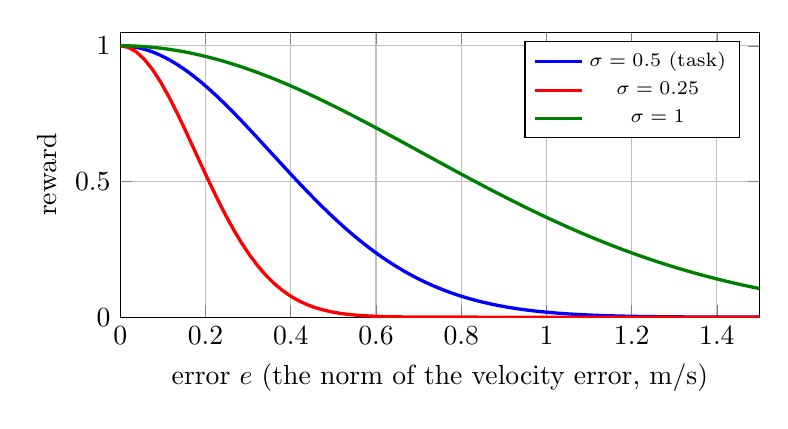
\begin{tikzpicture}
\begin{axis}[width=0.8\linewidth,height=5.2cm,xlabel={error $e$ (the norm of the velocity error, m/s)},ylabel={reward},xmin=0,xmax=1.5,ymin=0,ymax=1.05,grid=both,legend style={font=\scriptsize,at={(0.97,0.97)},anchor=north east},samples=80]
 \addplot[blue,very thick,domain=0:1.5] {exp(-x^2/0.25)};
 \addplot[red,very thick,domain=0:1.5] {exp(-x^2/0.0625)};
 \addplot[green!50!black,very thick,domain=0:1.5] {exp(-x^2/1.0)};
 \legend{$\sigma=0.5$ (task),$\sigma=0.25$,$\sigma=1$}
\end{axis}
\end{tikzpicture}
\captionof{figure}{The kernel $\exp(-e^2/\sigma^2)$. With the value of the task, $\sigma=0.5$, an error of $0.5$\,m/s gives the reward $e^{-1}=0.37$ and an error of $0.1$\,m/s gives $0.96$. A small $\sigma$ (red) is strict but gives almost no signal when the robot is still far from the target; a large $\sigma$ (green) is generous and hardly separates a good walk from a mediocre one.}
\end{center}

\begin{example}
The command is $(0.6,\,0)$\,m/s. The robot moves with $(0.4,\,0.1)$\,m/s and $v_z=0.05$\,m/s. The squared error is $0.04+0.01+0.0025=0.0525$, so the term is $\exp(-0.0525/0.25)=\exp(-0.21)=0.81$; with the weight $2$ this contributes $1.62$ to the reward of this step. If the robot walks with $0.2$\,m/s instead of $0.4$, the error is $0.16+0.01+0.0025=0.1725$ and the term is $\exp(-0.69)=0.50$.
\end{example}

\subsection*{The reward terms of the configuration}
\begin{center}
\small
\begin{tabular}{p{3.3cm}p{7.2cm}r}
\hline
term & meaning & weight\\
\hline
track linear velocity & kernel above, $\sigma=0.5$ & $+2.0$\\
track heading & kernel on the heading error, $\sigma\approx0.71$ & $+2.0$\\
upright & trunk stays vertical, kernel with $\sigma\approx0.45$ & $+1.0$\\
pose & joints stay near the default pose, with a tolerance that depends on the speed (standing, walking, running) & $+1.0$\\
joint position limits & penalty when a joint is near its limit & $-1.0$\\
action rate & squared change of the action between steps & $-0.1$\\
others (air time, clearance, slip, landing, self collision) & defined in the code, weight $0$ by default, set per robot & \\
\hline
\end{tabular}
\end{center}
If every positive term is perfect, the reward per step is $2+2+1+1=6$. The \textbf{penalties} are small; their job is to shape the \emph{style}: the action rate keeps the motion smooth (and so the torques low and the real motors happy), the limits keep the joints away from the hard stops, and the pose term keeps the robot from adopting a strange but fast gait. The tracking terms say \emph{what} to do, the rest says \emph{how}. The pose tolerance is a good design: when the command is zero (standing) the tolerance is tight, so the legs do not wander; when running it is loose, because large joint movements are needed.

\begin{aibox}[The reward design of Chapter~\ref{ch:rl5} in practice]
The advice of Part~\ref{part:rl} was: reward what you want, keep the reward bounded, add penalties for what you do not want, and check each term. In mjlab the check is built in: every term is logged separately, so after a few hundred iterations you can see which term dominates. A typical failure: the penalties are too large, the robot learns to stand still (the penalty-free policy) and the velocity reward stays low. The cure is to reduce the penalties, \emph{not} to increase the tracking weight.
\end{aibox}

\section*{Randomisation: so that it also works on the floor of the hall}
The configuration randomises the world, as in Chapter~\ref{ch:rl6}:
\begin{itemize}[nosep]
 \item \textbf{Pushes} every $1$ to $3$ seconds: the velocity of the robot is set to a random value (up to $\pm0.5$\,m/s horizontally, $\pm0.4$ vertically and $\pm0.52$\,rad/s in roll and pitch). The robot learns to recover.
 \item \textbf{Friction} of the feet from $0.3$ to $1.2$ (at start-up; all foot geometries get the same value).
 \item \textbf{Encoder bias} of $\pm0.015$\,rad for every joint: the robot learns not to trust the zero position of a joint completely.
 \item \textbf{Centre of mass} of the base shifted by up to $\pm2.5$\,cm in $x$ and $y$ and $\pm3$\,cm in $z$: the real centre of mass is never exactly where the model says (Chapter~\ref{ch:ctl2}).
 \item A random start: position $\pm0.5$\,m, direction anywhere in $[-\pi,\pi]$, at a height of $1$ to $5$\,cm.
\end{itemize}
These are the randomisations of the part of the configuration I read; a real project adds more (the masses of the links, the delay between command and torque, the motor strength).

\subsection*{A curriculum on the commands}
The velocity task has a \textbf{curriculum} (a function in the code that changes the ranges of the command during training): the robot first learns to follow small velocities and the limits are then increased as it does well. The principle is that a robot that cannot yet stand has no use for the command $1$\,m/s.

\begin{keyidea}[Summary]
\begin{itemize}[nosep]
 \item Velocity tracking: a command $(v_x,v_y,\omega_z)$ with a heading target, drawn every $3$--$8$\,s, with $10\%$ standing and $20\%$ sideways in the configuration read.
 \item The actor sees noisy, measurable values; the critic also sees privileged ones.
 \item Actions are scaled joint targets; the scale is smaller for the joints where mistakes hurt.
 \item Rewards: exponential kernels for the tracking ($\sigma$ is the tolerance) plus small penalties for the style; log every term.
 \item Randomise pushes, friction, encoder bias and the centre of mass; use a curriculum for the command range.
\end{itemize}
\end{keyidea}

\section*{Practice problems}
\begin{enumerate}[label=\textbf{\thechapter.\arabic*}]
  \item Compute the kernel $\exp(-e^2/\sigma^2)$ with $\sigma=0.5$ for the errors $0.1,\,0.25,\,0.5$ and $1$\,m/s. At which error is the reward exactly $0.5$ for $\sigma=0.5$?
  \item Choose $\sigma$ so that the reward is $0.5$ at the error $0.3$\,m/s. How large is it at $0.1$\,m/s?
  \item Command $(0.6,0)$, actual velocity $(0.5,\,0.1)$ and $v_z=0.05$ (all m/s). Compute the velocity reward term (with $\sigma=0.5$) and its contribution with the weight $2$. Repeat for command $(0,0.2)$ and actual $(0.1,\,0.25)$ with $v_z=-0.02$.
  \item The heading error is $0.4$\,rad. Compute the commanded turning rate ($0.5\cdot e$, clipped at $\pm0.5$) and the reward with $\sigma_h^2=0.5$. What happens to the commanded rate for the error $1.5$\,rad?
  \item Assume the robot follows the commanded turning rate exactly. How long does it need to turn from the heading error $1.2$\,rad to an error below $0.05$\,rad? (Write a loop or solve the differential equation of the unclipped part.)
  \item Explain why the pose term has a speed-dependent tolerance. What would happen with a tight tolerance when the command is $1$\,m/s?
  \item The action scale of the ankle roll is $0.45$ and that of the knee $1.0$. The network output is $\pm1$. What are the ranges of the joint target in radians around the default pose? What is the reason for the smaller value at the ankle?
  \item Suppose the penalties are so large that the total reward per step is mostly negative. Describe the policy that PPO will find, and what you would do. How could you see it in the logs?
  \item Modify the command program so that $20\%$ of the commands are standing and the maximum forward speed grows linearly from $0.2$ to $1.0$\,m/s over a curriculum of $10$ stages. Print the fraction of standing time and the maximum $|v_x|$ per stage over many samples.
  \item[\textbf{\thechapter.10}$\star$] Design a velocity-tracking configuration for the K1 on paper: list the observation terms of the actor and of the critic, the action scale per joint group, the reward terms with weights (start from the table), the randomisations and the termination conditions. For each choice write one sentence of justification, and mark which of them you would measure on the real robot first (Chapter~\ref{ch:mj4}).
\end{enumerate}
